% !TEX program = xelatex

\documentclass[hidelinks, 12pt, a4paper]{article}

\usepackage{fontspec}
\setmainfont[Ligatures=TeX]{Linux Libertine O}

\usepackage[hidelinks, colorlinks = true, urlcolor = blue]{hyperref}

\usepackage{indentfirst}
\usepackage{graphicx}
\usepackage[left=2cm,right=2cm,top=2cm,bottom=2cm]{geometry}
\usepackage{lipsum}
\usepackage{caption}
\usepackage{subcaption}



\begin{document}
\sloppy % this is legendary

\begin{titlepage}

\begin{figure}[h!]
  \begin{center}
    
\includegraphics[width=3cm]{assets/auth.pdf}
    \label{fig:cover_auth_logo}
  \end{center}
\end{figure}

\centering
\Large Αριστοτέλειο Πανεπιστήμιο Θεσσαλονίκης\\
\Large Πολυτεχνική Σχολή\\
%\large Τμήμα Ηλεκτρολόγων Μηχανικών και Μηχανικών Υπολογιστών\\
%\large Τομέας Τηλεπικοινωνιών

\vspace{\fill}

\LARGE \textbf{Java socket programming} \\
\LARGE \textbf{Δίκτυα 2}

\vspace{\fill}

\Large Θεόδωρος Κατζάλης \\
\Large ΑΕΜ:9282 \\ 
\Large katzalis@auth.gr

\vspace{\fill}
\raggedright

\centering
\vspace{\fill}
\today

\end{titlepage}

%\maketitle


\pagebreak
\tableofcontents
\pagebreak

% \section{Lorem}
% \lipsum


\section{Εισαγωγή}

Η συγκεκριμένη εργασία αποσκοπεί στην εξοικείωση εννοιών σχετικά με τα δίκτυα υπολογιστών τόσο σε θεωρητικό όσο και σε πρακτικό επίπεδο. Αυτό εξασφαλίζεται με την δημιουργία δικτυακών εφαρμογών χρησιμοποιώντας την γλώσσα προγραμματισμού \textbf{java} σε συνεργασία με τον server ithaki του μαθήματος με IP 155.207.18.208. Αυτή λοιπόν η συνεργασία επιτρέπει \textbf{active} έλεγχο και καθορισμό ορισμένων παραμέτρων αλλά και \textbf{passive} συλλογή δεδομένων επειτα απο συγκεκριμένα request του χρήστη στον server. Προς το τέλος αυτου του report θα γίνει αναφορά για πρωτόκολλα UDP και audio streaming.

Ενδεικτικά θα σημειώσουμε τις εφαρμογές που βασιστήκαμε για να συλλέξουμε πληροφορίες απο την πλευρά του client με μια σύντομη περιγραφή τους. Η πλειοψηφία αυτών βασίζεται στο πρωτόκολλο UDP:
\begin{itemize}
    \item \textbf{Echo}.
        Αποστολή μηνύματος της μορφής ΕΧΧΧX και λήψη πακέτου με δεδομένα που αφορούν την τρέχουσα ημερομηνία και ώρα.
    \item \textbf{Image}.
        Αποστολή μηνύματος της μορφής ΜΧΧΧΧ και λήψη πακέτων που περιλαμβάνουν το byte content μιας φωτογραφίας jpg. The challenge: Βρες τους delimiters, την αρχή και το τέλος της εικόνας 
    \item \textbf{Audio}.
        Αποστολή μηνύματος της μορφής ΑΧΧΧΧ και λήψη πακέτων ήχου κωδικοποιημένα σε DPCM και AQ-DPCM. The challenge: Κατανόσηση της κωδικοποίσης/αποκωδικοποίησης και βελτίωση της ποιότητας του ήχου.
    \item \textbf{Ithakicopter}. Συλλογή τηλεμετρίας απο custom κατασκευή προσομοίωσης ελικοπτέρου. The challenge: Autopilot
    \item \textbf{Car vehicle diagnostics}. Συλλογή διαγνωστικών στοιχείων απο μια βάση δεδομένων σχετικά με κάποια στοιχεία λειτουργίας ενός αυτοκινήτου. The challenge: Υλοποίηση υπολογισμού δεδομένων και εισαγωγή στο πρωτόκολλο TCP και τα streams.
\end{itemize}


Όσον αφορά τα διαγράμματα που χρησιμοποιήθηκαν στα session1.pdf και session2.pdf, για λόγους πληρότητας, θα αναφέρουμε ότι τα ιστογράμματα έγιναν με την χρήση του λογισμικού στατιστικής SPSS και όλα τα υπόλοιπα με την χρήση της βιβλιοθήκης matplotlib της γλώσσας προγραμματισμού python! 

Ακόμη στα πλαίσια του \textbf{statement of originality}, έχουμε παραθέσει βιβλιογραφία για τις πηγές στις οποίες βασιστήκαμε για να φέρουμε εις περας αυτήν την εργασία. Στο κομμάτι του κώδικα, αρχικός κόμβος ερεθισμάτων αποτέλεσε η αναφορά του ίδιου του μαθήματος. Οπότε θα την παραθέσουμε και πρώτη\cite{ergasia2}.
\section{Session 1}


Σχετικά με την χρονοκαθυστέρηση και την ρυθμαπόδοση των echo packets έχουμε να αναφέρουμε τα εξής:

\subsection{Echo packets Delay: ON}

\subsubsection{Χρόνος απόκρισης}
\begin{itemize}
    \item Μέση τιμή: 1815 milliseconds και τυπική απόκλιση: 557 milliseconds
    \item Αρκετά υψηλή η δεύτερη σε σύγκριση με την πρώτη το οποίο υποδηλώνει ότι τα δείγματα μεταξύ τους δεν είναι "συμπυκνωμένα"και αποκλίνουν σημαντικό βαθμό απο την μέση τιμή.
    \item Δεν φαίνεται με ξεκάθαρο τρόπο ποια κατανομή ακολουθούν τα δεδομένα μας, ωστόσο με κάποια επιφύλαξη θα μπορούσαμε να ισχυριστούμε ότι ακολουθούν bimodal κατανομή. Αυτό το συμπέρασμα προέκυψε απο την τάση να σχηματιστούν δύο καμπάνες.
\end{itemize}

\subsubsection{Ρυθμαπόδοση}

\begin{itemize}
    \item Μέση τιμή: 109 bits/sec και τυπική απόκλιση: 30.04 bits/sec
    \item Ομοίως με την μελέτη της χρονικής απόκρισης, η τυπική απόκλιση είναι αρκετά υψηλή, περίπου το 30\% της μέσης τιμής.
    \item Σχετικά με την κατανομή θα μπορούσαμε να υποστηρίξουμε ότι είναι μια right skew κατανομή μιας και παρουσιάζει μια ασυμμετρία γύρω απο την μέγιστη τιμή.
\end{itemize}
Παρατηρώντας το διάγραμμα της \textbf{ρυθμαπόδοσης} (throughput) διακρίνουμε ότι το εύρος τιμών κυμαίνεται περίπου απο 70 μέχρι 180 bits/second. Αξίζει να σημειωθούν κάποιες σχεδιαστικές αποφάσεις οι οποίες λήφθηκαν κατα τη διάρκεια υλοποίησης του αλγορίθμου της ρυθμαπόδοσης:

Σύμφωνα με την περιγραφή της άσκησης, ο υπολογισμός έπρεπε να γίνει με την τεχνική του κινούμενου μέσου όρου. Επιλέξαμε τα 8 δευτερόλεπτα ως το χρονικό πλαίσιο λήψης δεδομένων για κάθε δείγμα ρυθμαπόδοσης το οποίο υπολογίζεται για κάθε δευτερόλεπτο σε μήκος 4 συνεχόμενων λεπτών λήψης echo packets. Συνεπώς για τα τελευταία 8 δευτερόλεπτα απο τα 4 λεπτά της συνολικής μέτρησης δεν έχουν υπολογιστεί δείγματα ρυθμαπόδοσης. 

Η ύπαρξη των spikes στο διάγραμμα ερμηνεύεται απο το αν πρόλαβε κάποιο πακέτο στο πλαίσιο των 8 δευτερολέπτων να συμπεριληφθεί στο ένα δείγμα και όχι στο άλλο. Για παράδειγμα, αν έρθει ένα πακέτο την χρονική στιγμή $t_1 = t + 6.5$ second, και το επόμενο έρθει την χρονική στιγμή $t_2 = t + 8.1$, τότε το δείγμα της ρυθμαπόδοσης που μετρόυσε στο εύρος $[t, t+8]$ δεν θα λάβει υπόψιν το πακέτο που έφτασε στα $t + 8.1$. Ωστόσο στο δείγμα της ρυθμαπόδοσης με εύρος μέτρησης $[t+8, t+16]$ θα συμπεριληφθεί η τιμή του. Συγκεκριμένα, η τιμή αυτή είναι $32*8$ bits, αφού το κάθε echo packet response περιέχει 32 bytes\footnote{Ο τρόπος με τον οποίο διαπιστώσαμε το μέγεθος των δεδομένων έγινε με την βοήθεια του wireshark} δεδομένα. Για αυτό μπορούμε να παρατηρήσουμε ότι τα spikes διαφέρουν απο τα υπόλοιπα δείγματα πολλαπλάσια του $32$. Σε μια zoom out έκδοση του γραφήματος θα φαινόταν σίγουρα μια πιο ομαλή καμπύλη.


\subsection{Echo packets Delay: OFF}

\subsubsection{Χρόνος απόκρισης}
Στην συγκεκριμένη περίπτωση η χρονοκαθυστέρηση των δειγμάτων μειώνεται αισθητά σε χαμηλότερες τιμές milliseconds με αποτέλεσμα να λαμβάνουμε αρκετά περισσότερα δείγματα συγκριτικά με την προηγούμενη περίπτωση. Συνεπώς για λόγους ευκρίνειας\footnote{engineering appreciation όπως έχει ειπωθεί και στο μάθημα} παραθέτουμε μια zoom in εκδοχή του διαγράμματος του χρόνου απόκρισης με εύρος ενδεικτικά 100-200 packets. Σε γενικές γραμμές το εύρος της χρονοκαθυστέρησης κυμαίνεται απο 230-260 milliseconds. Πιο συγκεκριμένα έχουμε:
\begin{itemize}
    \item Μέση τιμή: 237 milliseconds και τυπική απόκλιση: 7 milliseconds 
    \item Συγκριτικά με Delay: ON, βλέπουμε ότι η τυπική απόκλιση είναι αρκετά μικρή σε σχέση με την μέση τιμή, επομένως τα δείγματα δεν έχουν την τάση να είναι "αραιωμένα".
    \item Σχετικά με την κατανομή μπορούμε να διακρίνουμε την δημιουργία δύο στενών καμπανών γύρω απο τις τιμές 232 και 246. Συνεπώς θα μπορούσαμε να ισχυριστούμε για μια ακόμη φορά bimodal distribution. 
\end{itemize}

\subsubsection{Ρυθμαπόδοση}
Για τις σχεδιαστικές αποφάσεις καθως και την ερμηνεία των spikes, έχει γίνει ήδη αναφορά στην προηγούμενη ανάλυση (Delay: ON).

Όπως έχει αναφερθεί, ο αριθμός των πακέτων που φτάνουν στον δέκτη είναι πολύ μεγαλύτερος με μικρότερη χρονοκαθυστέρηση μεταξύ των πακέτων, συνεπώς η ρυθμαπόδοση αυξάνεται αισθητά.
\begin{itemize}
    \item Μέση τιμή: 1040 bits/sec και τυπική απόκλιση: 18 bits/sec.
    \item Εξίσου μικρή η τυπική απόκλιση συγκριτικά με την μεση τιμή.
    \item Σχετικά με τη κατανομή μιας και οι τιμές συγκεντρώνεται στο αριστερό κομμάτι του γραφήματος θα μπορούσαμε να υποθέσουμε λογαριθμική κατανομή.
\end{itemize}


'Οσα έχουν αναφερθεί μέχρι στιγμής αφορούν τον σχολιασμό των διαγραμμάτων G1-G8.

\subsection{Retransmission timeout (RTO)}


Για λόγους γρήγορης και αξιόπιστης επικοινωνίας σχετικά με το πρωτόκολλο TCP, υπάρχει η ανάγκη πρόβλεψης και επαναπροσδιόρισης των παραμέτρων timeout σε ένα σύστημα επικοινωνίας. Πόσο πρέπει να περιμένει ο sender αν δεν λάβει  ACK απο τον receiver για να ξαναστείλει την πληροφορία; Ο προσδιορισμός των timers είναι λοιπόν πολύ σημαντικός διότι αν δεν ρυθμιστεί σωστά, υπάρχει η πιθανότητα να ξαναστείλουμε πακέτα πολύ γρήγορα προτού ο δέκτης να προλάβει να στείλει ACΚ ή το ανάποδο, δηλαδή να περιένουμε πολύ να ξαναστείλουμε ένα πακέτο\cite{gfg_rto, saminir}. 

Υπάρχουν κάποιες μαθηματικές σχέσεις οι οποίες υπολογίζουν τον retransmssion timer και υπάρχουν συγκεκριμένα 3 σταθερές α, β και γ. Εμείς επιλέξαμε αρχικά σταθερά τα α και β με τιμές $1 - 1/8 = 0.875$ και $1 - 1/4 = 0.750$. Εσκεμμένα γράψαμε με αυτήν την μορφή τις εξισώσεις προκειμένου να είμαστε συμβατοί με το notation των εξισώσεων που μας δίνονται στα πλαίσια του μαθήματος, μιας και οι αναφορές\cite{rfc}, τα δικα μας α και β, τα συμβολίζουν ως (1-α) και (1-β). Για την επιλογή του γ (k σύμφωνα με RFC) δοκιμάσαμε στην αρχή την προτεινόμενη τιμή 4. Στη συνέχεια παρατηρώντας το γράφημα R1 προσπαθούσαμε να φτάσουμε την γραμμή RTO να αγκαλιάζει το RTT, δηλαδή να μην είναι πολύ πάνω αλλά και ούτε απο κάτω του RTT. Τελικά επιλέξαμε την τιμή 1,8 και βλέπουμε ότι ικανοποιητικά η γραμμή RTO ακολουθεί σωστά το RTT.

\subsection{Tone frequency}

Γνωρίζουμε ότι η εικονική γεννήτρια συχνοτήτων παράγει δύο ημίτονα και στέλνει την πληροφορία με κωδικοποίηση DPCM. Χρησιμοποιώντας το εργαλείο audacity, προκειμένου να βρούμε τις συχνότητες, παρατηρώντας τα spikes του spectrum plot, μπορούμε να εικάσουμε επιλέγοντας τις υψηλότερες κορυφές, ότι οι συχνότητες των ημιτόνων είναι 421 και 343 Hz.

\begin{figure}[h!]
\centering
	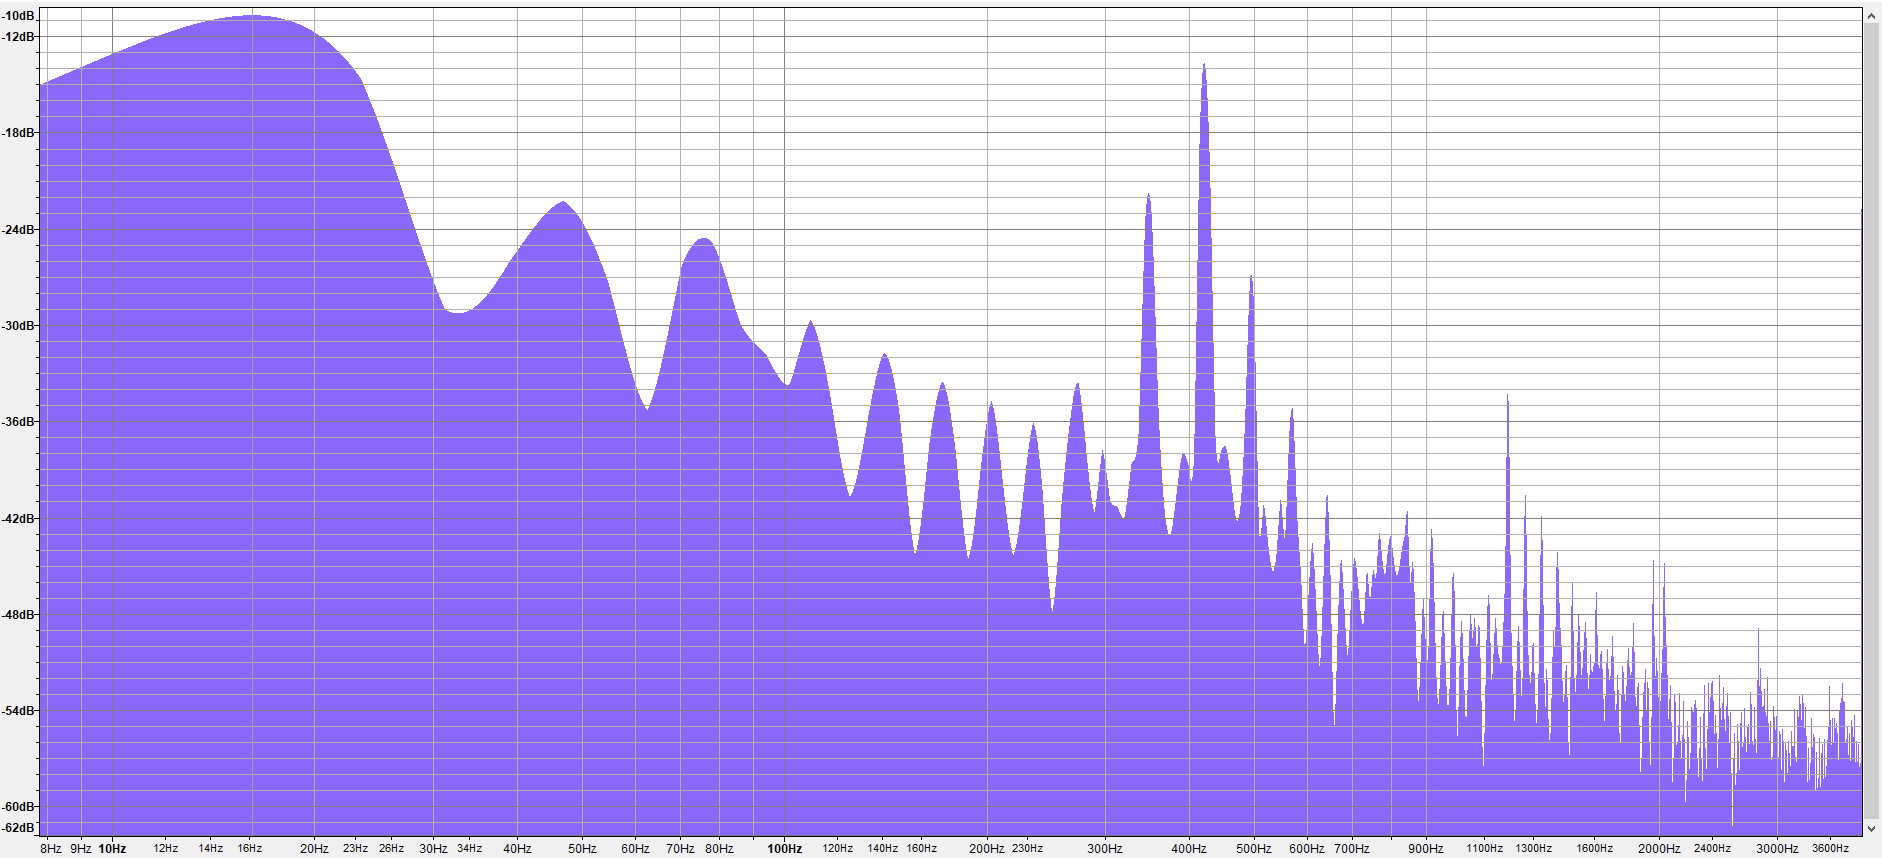
\includegraphics[height=.3\textheight, width=\textwidth]{assets/session1/spectrum.png}
    \caption{Frequency spectrum απο δείγμα της εικονικής γεννήτριας συχνοτήτων}
\end{figure}

\subsection{Image}

Κατά τη διάρκεια ανάπτυξης της εφαρμογής της εικόνας. στην προσπάθεια μας να δημιουργήσουμε real-time video, αλλάξαμε το μέγεθος των πακέτων απο 128 σε 1024 bytes χρησιμοποιώντας το κατάλληλο request code και καταφέραμε λαμβάνοντας 100 δείγματα να δημιουργήσουμε ένα βίντεο 40 δευτερολέπτων κάνοντας merge τα δείγματα αυτά. Το video μπορείτε να το δείτε \href{https://drive.google.com/file/d/1yfwckvGBr8YteigF3ainMJMXwLOzjZ9u/view?usp=sharing}{εδώ}. Αξίζει να σημειωθεί οτι για το βίντεο χρησιμοποιήσαμε την κάμερα FIX. Θα μπορούσαμε να χρησιμοποιούσαμε την PTZ για να είχαμε πιο πιστευτή πραγματική αναπαράσταση μιας και ο χρόνος λήψης της εικόνας είναι πιο μικρός εξαιτίας της μικρότερης ανάλυσης της.

Σχετικά με τον χρόνο που αποτυπώνουν οι εικόνες, παρατηρήσαμε οτι στην FIX η ημερομηνία και η ώρα είναι ακριβής, ενώ στην PTZ υπάρχει μια καθυστέρηση της τάξης των 4 λεπτών περίπου. Φυσικά με κατάλληλες εντολές DIR=X, υπάρχει και η δυνατότητα απεικόνισης του πύργου του ΟΤΕ (session 2)!

Σχετικά με την υλοποίηση  της λήψης της εικόνας, ελέγχουμε σε κάθε πακέτο που λαμβάνουμε αν υπάρχει ο delimiter \textbf{OxFF D9}. Αυτή η πληροφορία θα σηματοδοτούσε το τέλος της εικόνας και έπειτα γράφοντας τα δεδομένα σε ένα αρχείο jpg, υπάρχει η δυνατότητα προβολής. Ωστόσο, αξίζει να αναφέρουμε ότι εξαιτίας ενδεχομένως θορύβου κβάντισης και καναλιού, αυτός ο delimiter μπορεί να μην εντοπιστεί. Βέβαια σε πρώιμες υλοποιήσεις, στις οποίες δεν ελέγχαμε αν υπήρχαν delimiters, αποθηκεύαμε όλη την πληροφορία και υπήρχε εξίσου η δυνατότητα προβολής (ακόμα και αν υπήρχαν περισσότερα bytes στο τέλος της εικόνας μετά τον delimiter OxFF D9). Μιας και δεν ειπώθηκε κάτι για τα bytes που σηματοδοτούν την έναρξη της εικόνας, παρατηρήσαμε απο το wireshark ότι η πρώτη πληροφορία που λαμβάνουμε είναι το OxFF D8 (start of image).

\subsection{Audio}

Σχετικά με τον ήχο χρησιμοποιήσαμε τους κωδικούς L22 και L11 (second clip AQ-DPCM) για τα ζητούμενα της εργασίας: 
\begin{itemize}
    \item L22:
    \item L11: 
\end{itemize}

Όσον αφορά τα γραφήματα του ήχου μπορούμε να παρατηρήσουμε το λεγόμενο \textbf{clipping effect}. Εξαιτίας της αναδρομικής σχέσης στην αποκωδικοποίηση DPCM και AQ-DPCM για την λήψη των πραγματικών δειγμάτων, υπάρχει περίπτωση οι τιμές των samples να υπερβούν τις μέγιστες και τις ελάχιστες των 8 και 16 bits προσημασμένου ακεραίου που χρησιμοποιήθηκαν για την κβάντιση τους. Οπότε προκειμένου να αποφύγουμε το ενδεχόμενο να γίνει roll back απο την μεγαλύτερη τιμή στην μικρότερη, κάθε φορά που ο integer (32 bits) ξεπερνούσε την μεγιστη τιμή ή την ελάχιστη τιμή των bits κωδικοποίσης, τότε το θέταμε ίσο με το μέγιστο ή το ελάχιστο αντίστοιχα. Για αυτό το λόγο επίσης μπορούσε να ερμηνεύσουμε και στο ιστόγραμμα, ιδιαίτερα υψηλές τιμές στις ελάχιστες όπου γινόταν το clipping.

Επειδή ο αριθμός των δειγμάτων είναι ιδιαίτερα υψηλός, έχουμε προσθέσει στα διαγράμματα ήχου και zoom in εκδοχές προκειμένου να έχουμε μια αίσθηση του τρόπου διακύμανσης των τιμών σε τοπικό επίπεδο. Ενδιαφέρον παρουσιάζει το διάγραμμα του τόνου, απο την εικονική γεννήτρια συχνοτήτων, στο οποίο μπορούμε να παρατηρήσουμε το σχηματισμό ενός ημιτονοειδούς σήματος!

Σχετικά με την μέση τιμή, η οποία προστίθεται στα δείγματα, έχει μικρή τιμή συγκριτικά με τις διαφορές των δειγμάτων οι οποίες καθορίζονται σε μεγάλο βαθμό απο τις μεγάλες τιμές του step.

Το request code audio που φαίνεται στο wireshark αντιστοιχίζεται στην κυματομορφή AQ-DPCM (G9), ενώ τα υπόλοιπα δείγματα έχουν ληφθεί για το ίδιο τραγούδι αλλά διαφορετικές χρονικές στιγμές.

\subsubsection{AQ-DPCM}

\begin{itemize}
    \item Το ιστόγραμμα των διαφορών των δειγμάτων για AQ-DPCM δείχνει μια τριγωνική/κανονική κατανομή και ένα απότομο spike. Οι τιμές των δειγμάτων έχουν υψηλές τιμές της τάξης των χιλιάδων με μέση τιμή -48 και τυπική απόκλιση κοντά στα 4000.
    \item Το ιστόγραμμα των ίδιων των σημάτων φαίνεται να ακολουθεί μια κανονική κατανομή με μέση τιμή -11600 και τυπική απόκλιση 10282. Το clipping effect συμβάλει στο spike του ιστογράμματος, καθώς πολλές τιμές που υπερβαίνουν τα όρια συγκεντρώνονται σε εκείνη την περιοχή, δηλαδή την ελάχιστη τιμή των 16 bits προσημασμένου ακεραίου.
\end{itemize}


\subsubsection{DPCM}

Το DPCM απο την άλλη πλευρά μας δείχνει δύο πολύ καθαρά γραφήματα όσον αφορά τις διαφορές των δειγμάτων και των ίδιων των δειγμάτων. Τα δεδομένα και στις δύο περιπτώσεις φαίνεται να ακολουθούν τριγωνική κατανομή. Αξίζει να σημειωθεί οτι οι τιμές είναι αρκετά πιο χαμηλές σε σύγκριση με το AQ-DPCM, μιας και θεωρούμε ότι το step είναι ίσο με 1, σε αντίθεση με το AQ στο οποίο μας έρχεται ως πληροφορία το step και έχει και ιδιαίτερα υψηλές τιμές επηρεάζοντας σημαντικά τις διαφορές των δειγμάτων και ως συνεπακόλουθο και τα ίδια τα δείγματα.


\subsubsection{Ithakicopter - autopilot}

Σχετικά με το ithakicopter επιλέγοντας AUTOPILOT:ON, έχουμε την δυνατότητα να καθορίσουμε ένα flightlevel στο οποίο το copter προσπαθεί με σταθερό ρυθμό να φτάσει και να παραμείνει εκεί. Βλέποντας την καμπύλη του ALTITUDE στα γραφήματα φαίνεται η ανοδική πορεία, μια μικρή σταθεροποίηση και έπειτα η πτώση (πατώντας AUTOPILOT:OFF). 

Στην δεύτερη μας μέτρηση πειραματιστήκαμε λίγο παραπάνω και επιτηδευμένα στείλαμε προς τα κάτω το copter αφού είχαμε φτάσει στο επιθυμητό flightlevel, ωστόσο ο μηχανισμός autpilot έκανε σωστά την δουλεία του και προσπάθησε να το επαναφέρει.


\textbf{Ithakicopter αλλα TCP version}: Προσπαθήσαμε και εμείς με την δική μας σειρά αρχικά να στείλουμε εντολές μέσω TCP και κατ' επέκταση να προσπαθήσουμε να υλοποιήσουμε τον μηχανισμό autopilot. Κάτι το οποίο αξίζει να αναφερθεί είναι ότι την στιγμή δημιουργίας του TCP socket, χωρίς να υπάρξει κάποιο write, η ithaki μας έστελνε κάτι σαν εισαγωγικό μήνυμα το οποίο μας έλεγε κάποιες πληροφορίες για το format της εντολής που πρέπει να σταλθεί προκειμένου να έχει απόκριση ο server. Οπότε αυτά τα bits θα έπρεπε πρώτα να γίνουν skip, πρώτου γίνει προσπάθεια λήψης τηλεμετρίας μετά απο εντολή write. 

Στα πλαίσια λοιπόν του TCP ithakicopter, προσπαθήσαμε στη συνέχεια να υλοποιήσουμε το \textbf{autopilot}. Στην αρχή ο τρόπος με τον οποίο δημιουργήσαμε τις συναρτήσεις και τον σχεδιασμό της εργασίας, είχαμε μια ρουτίνα tcp η οποία και άκουγε αλλά και έστελνε πακέτα. Προκειμένου να έχουμε μια ρουτίνα η οποία μόνο θα ακούει και ανάλογα το feedback θα πρέπει να στέλνουμε νέα commands, αποφασίσαμε να χρησιμοποιήσουμε ήδη το  UDP passive κομμάτι τηλεμετρίας και το TCP μόνο όταν πρέπει να στείλουμε νέες τιμές στα moters για να ελέγχουμε το ύψος. Προς το παρόν δεν έχει γίνει κάποιος μαθηματικός υπολογισμός (θεωρία Συστημάτων Αυτομάτου ελέγχου) και ο autopilot το μόνο που μπορεί να κάνει είναι να να κρατάει τους moters σε ένα εύρος τιμών καθορισμένο απο δύο μεταβλητές. Δεν μπορέσαμε δηλαδή να βρούμε αντιστοίχιση επίδρασης moters σε altitude και σίγουρα η συγκεκριμένη υλοποίηση είναι αρκετά μακρυά απο αυτήν που υπάρχει ήδη! 

\subsubsection{Car vehicle diagnostics}

Η συγκεκριμένη εφαρμογή αποτέλεσε το έναυσμα ενασχόλησης με το TCP πρωτόκολλο και τα Input και Output streams. Αξίζει να σημειωθεί ότι στα αρχικά στάδια της εργασίας προσπαθώντας να χειριστούμε τα streams, συγκεκριμένα μάλιστα για το input, χρησιμοποιήσαμε την μέθοδο readAllBytes(). Με την κλήση αυτής της μεθόδου το πρόγραμμα σταματούσε για αρκετά δευτερόλεπτα περιμένοντας να συλλέξει δεδομένα απο το stream. Ωστόσο έπειτα απο μια τέτοια κλήση δεν υπήρχε η δυνατότητα με το ίδιο stream να γράψεις στο output και να ακούσεις ξανά. Σε κάθε τέτοια προσπάθεια λαμβάναμε null πακέτα. Χωρίς να είμαστε ιδιαίτερα σίγουροι γιατί συνέβαινε αυτό, μπορούμε να εικάσουμε ότι έκλεινε το stream και δεν μπορούσες να το ξαναχρησιμοποιήσεις. Ωστόσο χρησιμοποιώντας μεθόδους που διαβάζουν bits ή lines, δεν υπήρχε τέτοιο πρόβλημα και μάλιστα λαμβάνουμε τα δεδομένα πολύ γρήγορα χωρίς να υπάρχει κάποιου είδους αναμονή όπως γινόταν με το readAllBytes().  



\section{Section 2}

Στο session 2 επαναλάβαμε ακριβώς οτι είχαμε κάνει στο session 1 με διαφορά περίπου δύο ημερών. Δεν θα αναφέρουμε σχολαστικά τους συλλογισμούς μας, μιας και τα περισσότερα έχουν ειπωθεί στο session 1. Ωστόσο θα σημειώσουμε τα στοιχεία των γραφημάτων.

\subsection{Audio}

Για τα δεδομένα του session 2 στο κομμάτι του ήχου χρησιμοποιήσαμε τα κομμάτια L01 και L02. Αυτήν την φορά η κυματομορφή είναι κωδικοποίησης DPCM.

\begin{itemize}
    \item L01: Audio title
    \item L02; Audio title
\end{itemize}

\section{Tone frequency}

Μια αρκετά πιο καθαρή εικόνα σε σύγκριση με το plot spectrum στο session 1. Με παρόμοια λογική βλέποντας τις κορυφές εικάζουμε ότι οι συχνότητες είναι 1024 και 349 Hz.

\begin{figure}[h!]
\centering
	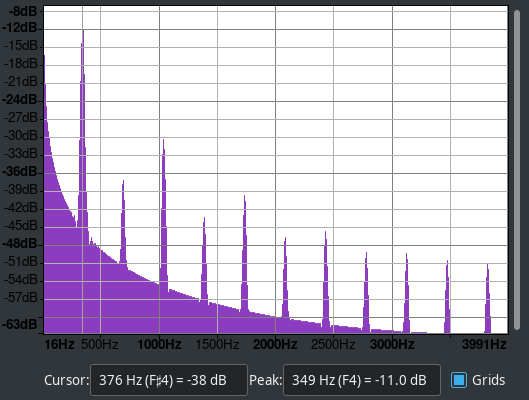
\includegraphics[height=.3\textheight, width=\textwidth]{assets/session2/spectrum.png}
    \caption{Frequency spectrum, 1042 Hz and 349 Hz}
\end{figure}


\pagebreak
\section{Ανάλυση πηγαίου κώδικα}

Σε γενικές γραμμές έχουμε ήδη αναφέρει κατα τη συγγραφή του report κάποια στοιχεία σχετικά με την συλλογιστική πορεία που ακολουθήσαμε για τον σχεδιασμό και την υλοποίηση των αλγορίθμων που απαιτούνται για την εργασία. Βασιστήκαμε σε πολλές πηγές και θα προσπαθήσουμε να παραθέσουμε κάποιες απο αυτές.

\begin{itemize}
    \item Μια γρήγορη ανακεφαλαίωση της γλώσσας προγραμματισμού java \cite{derek}
    \item Εισαγωγή σε Datagram Sockets \cite{romaniancoder, oracle}
    \item Πως να γράψεις byte array σε αρχείο; \cite{javafile}
    \item Μετατροπη byte σε hexadecimal \cite{programizhex}
    \item Εισαγωγή σε εφαρμογές ήχου χρησιμοποιώντας java \cite{oraclesound}
    \item Little endian και Big endian σε εφαρμογές ήχου \cite{stackendian}
    \item Πως να γράψω ήχο σε αρχείο \cite{stackaudiofile}
    \item Εισαγωγή σε TCP \cite{tutorpoints, mediumtcp, codejava}
    \item How to parse strings in java? \cite{stackparsestring}
\end{itemize}


Επίσης να σημειώσουμε ότι προσπαθήσαμε ως επι το πλειστον να κάνουμε καλή διαχείριση errors και try, catch blocks προκειμένου να εντοπίζουμε γρήγορα προβλήματα αλλά και να μην διακόπτεται η λειτουργία του προγράμματος για ενδεχομένως "ασήμαντα" errors.

\subsection{User Interface}

Προτού αναφερθούμε στα UDP και audio streaming protocols που έρχονται στη συνέχεια, θα θέλαμε να αναφέρουμε συνοπτικά το διαδραστικό menu του χρήστη για αισθητικούς αλλά και οργανωτικούς/πρακτικούς λόγους. Πιο συγκεκριμένα, την στιγμή έναρξης της java εργασίας παρουσιάζεται ένα "welcome logo\footnote{The so called ascii art!}" και παρακινεί τον χρήστη να πατήσει ENTER προκειμένου να ξεκινήσει η εργασία.

\begin{figure}[h!]
\centering
	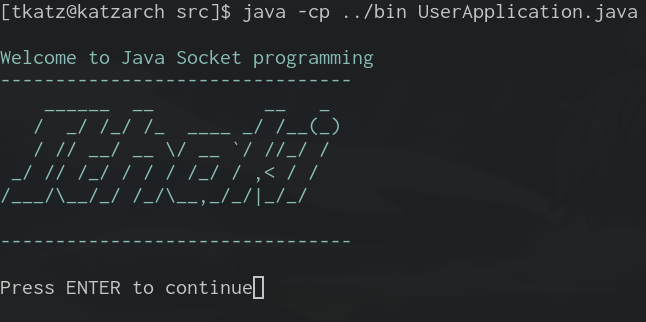
\includegraphics[height=.3\textheight, width=\textwidth]{assets/ui_welcome.png}
	\caption{Welcome screen!} 
    \label{fig:ui}
\end{figure}


Στη συνέχεια παρουσιάζεται μια λίστα με αριθμούς, όπου κάθε αριθμός αντιστοιχίζεται στην εκάστοτε εφαρμογή. Σε περίπτωση που η είσοδος είναι κάτι διαφορετικό απο αυτούς τους αριθμούς τότε ξανα ζητείται απο τον χρήστη να πατήσει έναν απο τους διαθέσιμους αριθμούς. Σε εφαρμογές όπως Ithakicopter UDP passive και στο autopilot που χρησιμοποιούμε το UDP άρα χρειαζόμαστε και το ithakicopter.jar, έχουμε blocking σημείο στο οποίο ζητάται απο τον χρήστη να ανοίξει το jar και να πατήσει ENTER για να συνεχίσει η εφαρμογή (όπως κάνουμε δηλαδή και στο welcome σημείο).

\begin{figure}[h!]
\centering
	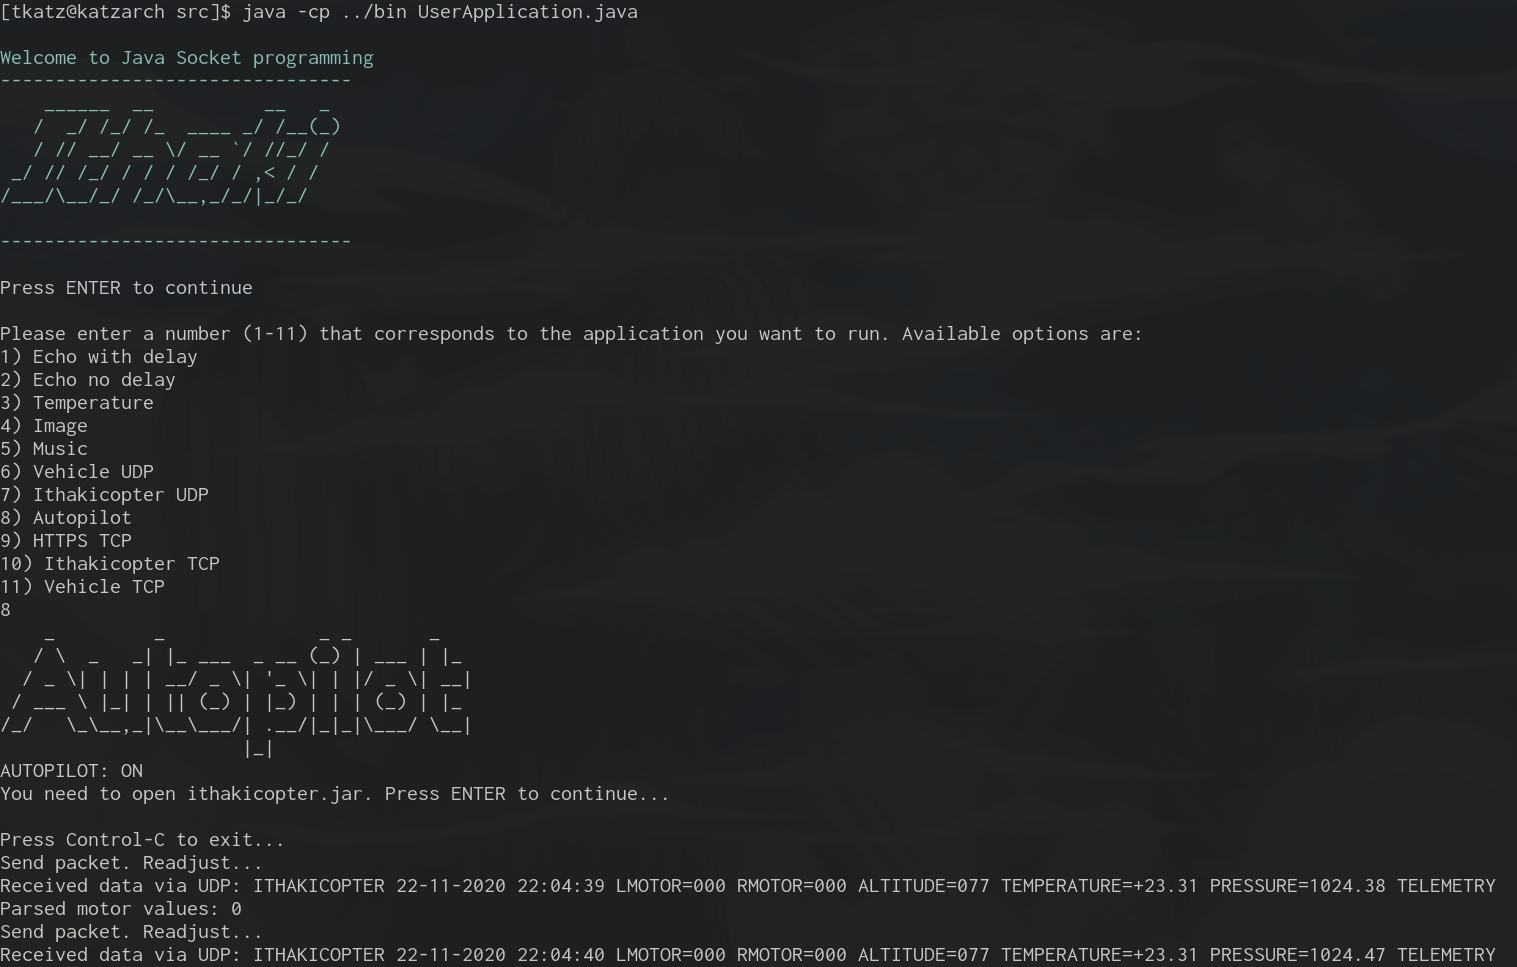
\includegraphics[height=.3\textheight, width=\textwidth]{assets/ui.png}
	\caption{Εκτέλεση προγράμματος σε κέλυφος Bash. Επιλογή Autopilot} 
    \label{fig:ui}
\end{figure}

% \begin{figure}
%      \begin{subfigure}[b]{.5\textwidth}
%          \centering
%          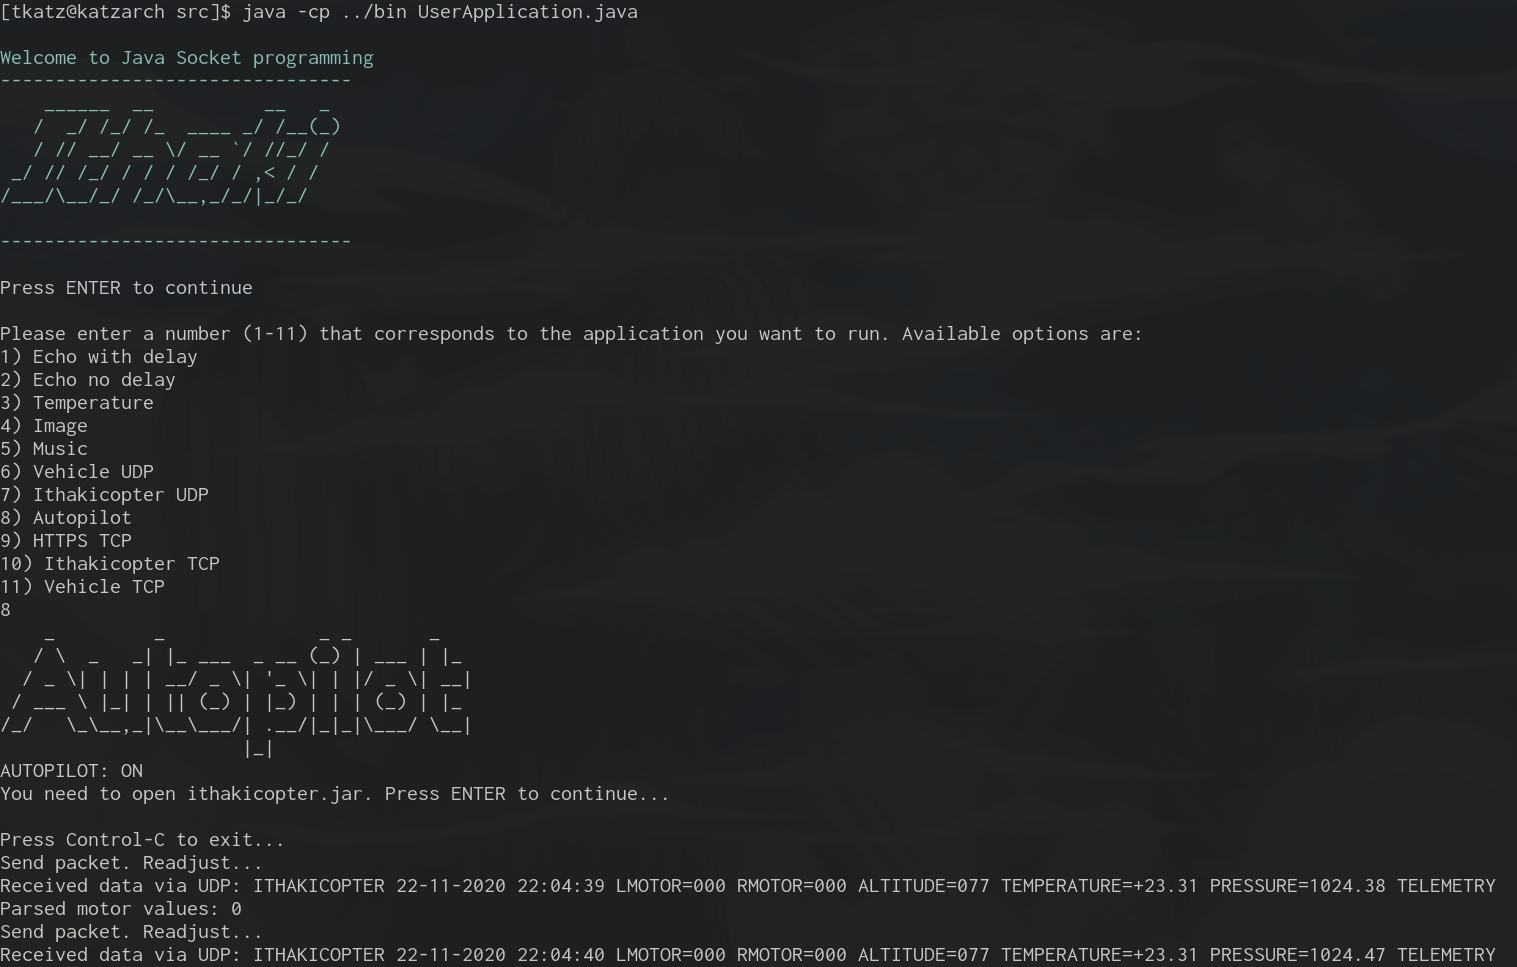
\includegraphics[width=\textwidth]{assets/ui.png}
%          \caption{$y=3sinx$}
%      \end{subfigure}
%      \hfill
%      \begin{subfigure}[b]{.5\textwidth}
%          \centering
%          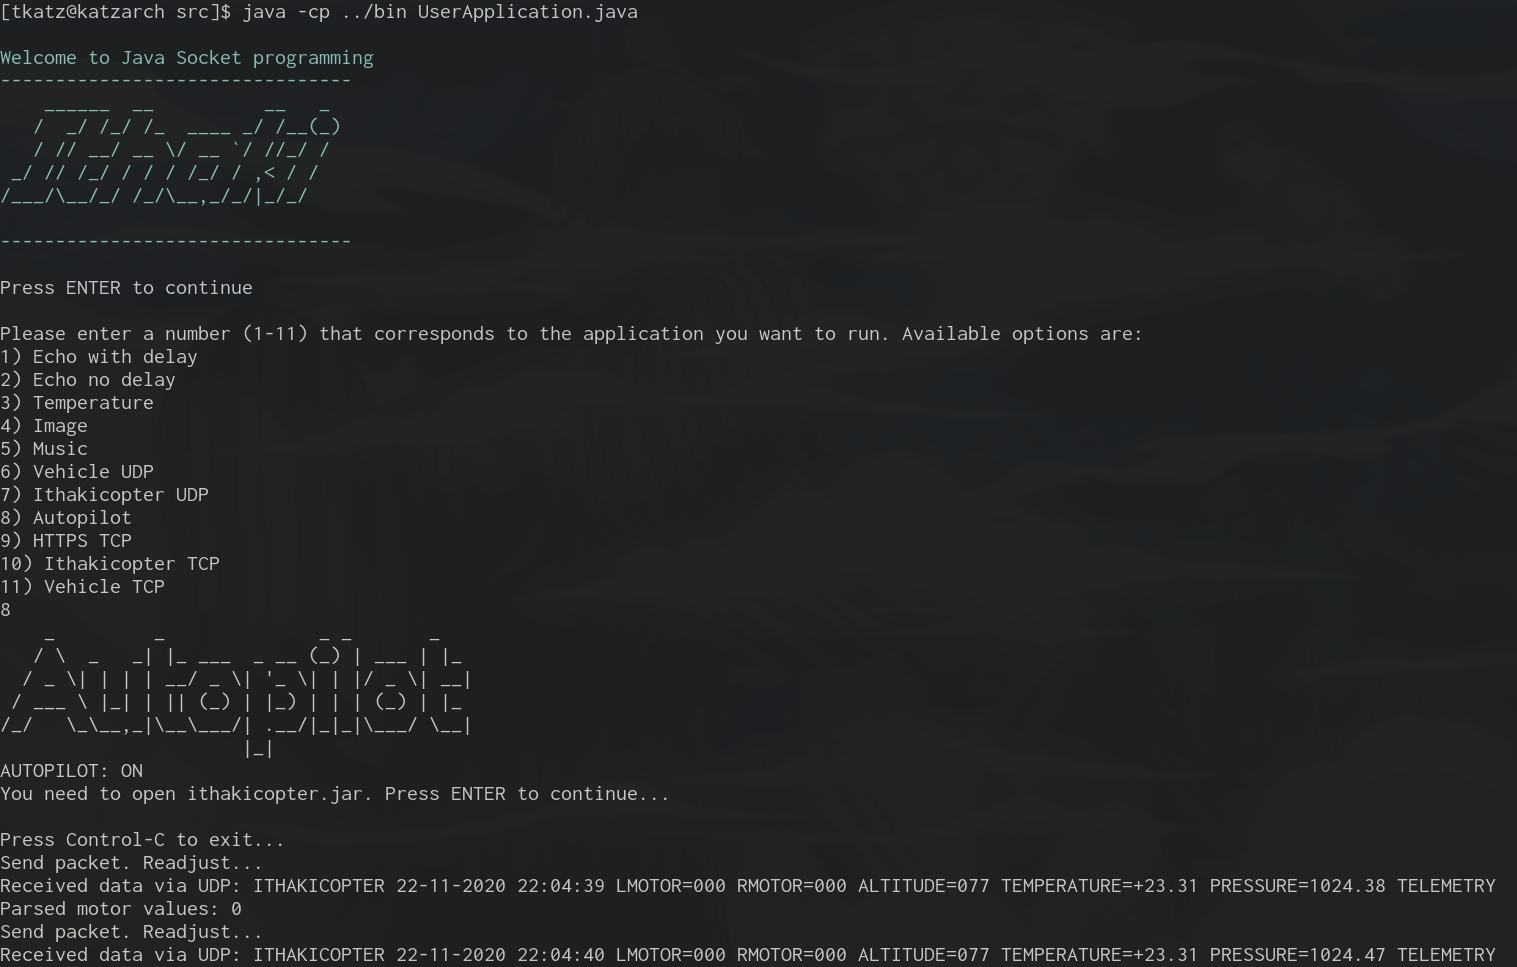
\includegraphics[width=\textwidth]{assets/ui.png}
%          \caption{$y=5/x$}
%      \end{subfigure}
%         \caption{Three simple graphs}
%         \label{fig:three graphs}
% \end{figure}


\section{UDP}
Here we are going to talk about UDP protocol.



\section{Audio streaming protocols}




\clearpage

\bibliographystyle{plain}
\bibliography{bib/bib.bib}

\end{document}
